\documentclass[11pt]{article}

\usepackage{natbib,rotfloat,epsfig,setspace,amssymb,amsmath, comment}
\usepackage{lscape}

\setlength{\hoffset}{0.01in}
\setlength{\voffset}{-0.6in}
\setlength{\textwidth}{6.0in}
\setlength{\evensidemargin}{0in}
\setlength{\oddsidemargin}{0in}
\setlength{\textheight}{8.5in}

\begin{document}

\onehalfspace

\title{Economics 512 -- Homework 7}
\author{Maxence Valentin}
\date{February 18, 2019}
\maketitle

\paragraph{Question 1.} See attached code and Figure 1 and 2.

\begin{figure}[!h]
	\centering
	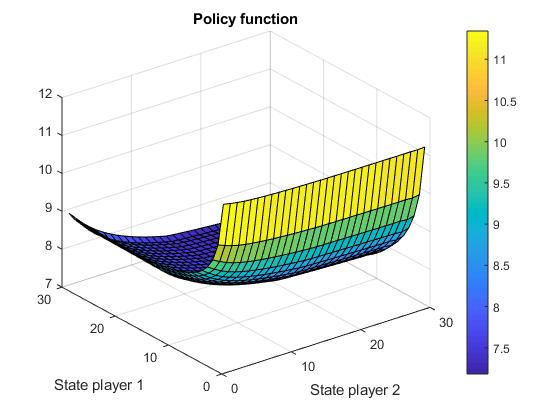
\includegraphics[width=0.8\textwidth]{Figures/figure1.jpg}
	\caption{Question 1a}
\end{figure}

\begin{figure}[!h]
	\centering
	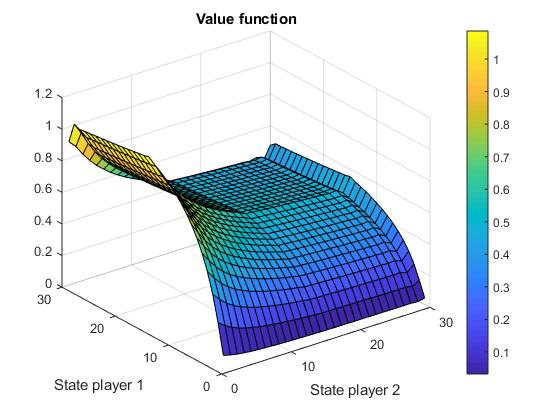
\includegraphics[width=0.8\textwidth]{Figures/figure2.jpg}
	\caption{Question 1b}
\end{figure}


\paragraph{Question 2.}  See attached code and Figure 3-5.

\begin{figure}[!h]
	\centering
	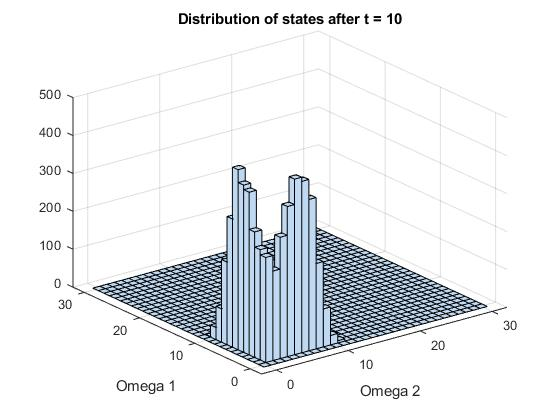
\includegraphics[width=0.8\textwidth]{Figures/figure3.jpg}
	\caption{Question 2a}
\end{figure}

\begin{figure}[!h]
	\centering
	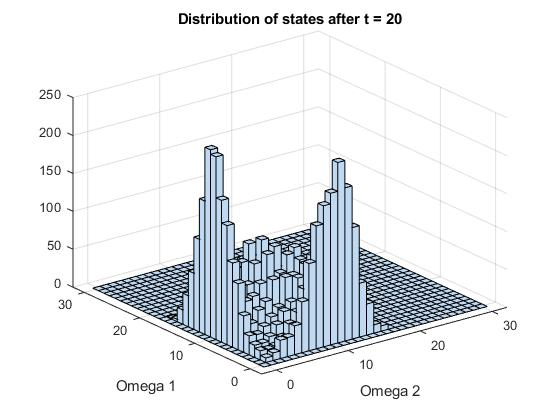
\includegraphics[width=0.8\textwidth]{Figures/figure4.jpg}
	\caption{Question 2b}
\end{figure}

\begin{figure}[!h]
	\centering
	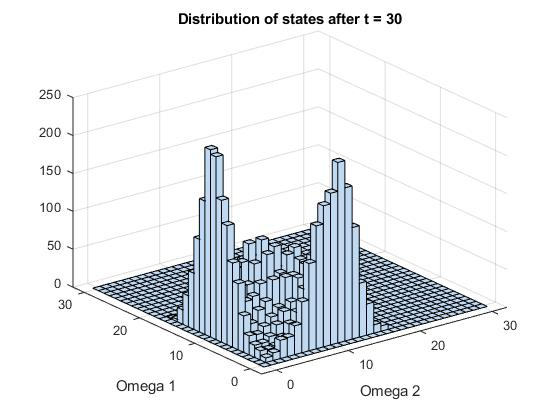
\includegraphics[width=0.8\textwidth]{Figures/figure5.jpg}
	\caption{Question 2c}
\end{figure}

\paragraph{Question 3.} See attached code and figure 6.

\begin{landscape}
\begin{figure}[!h]
	
	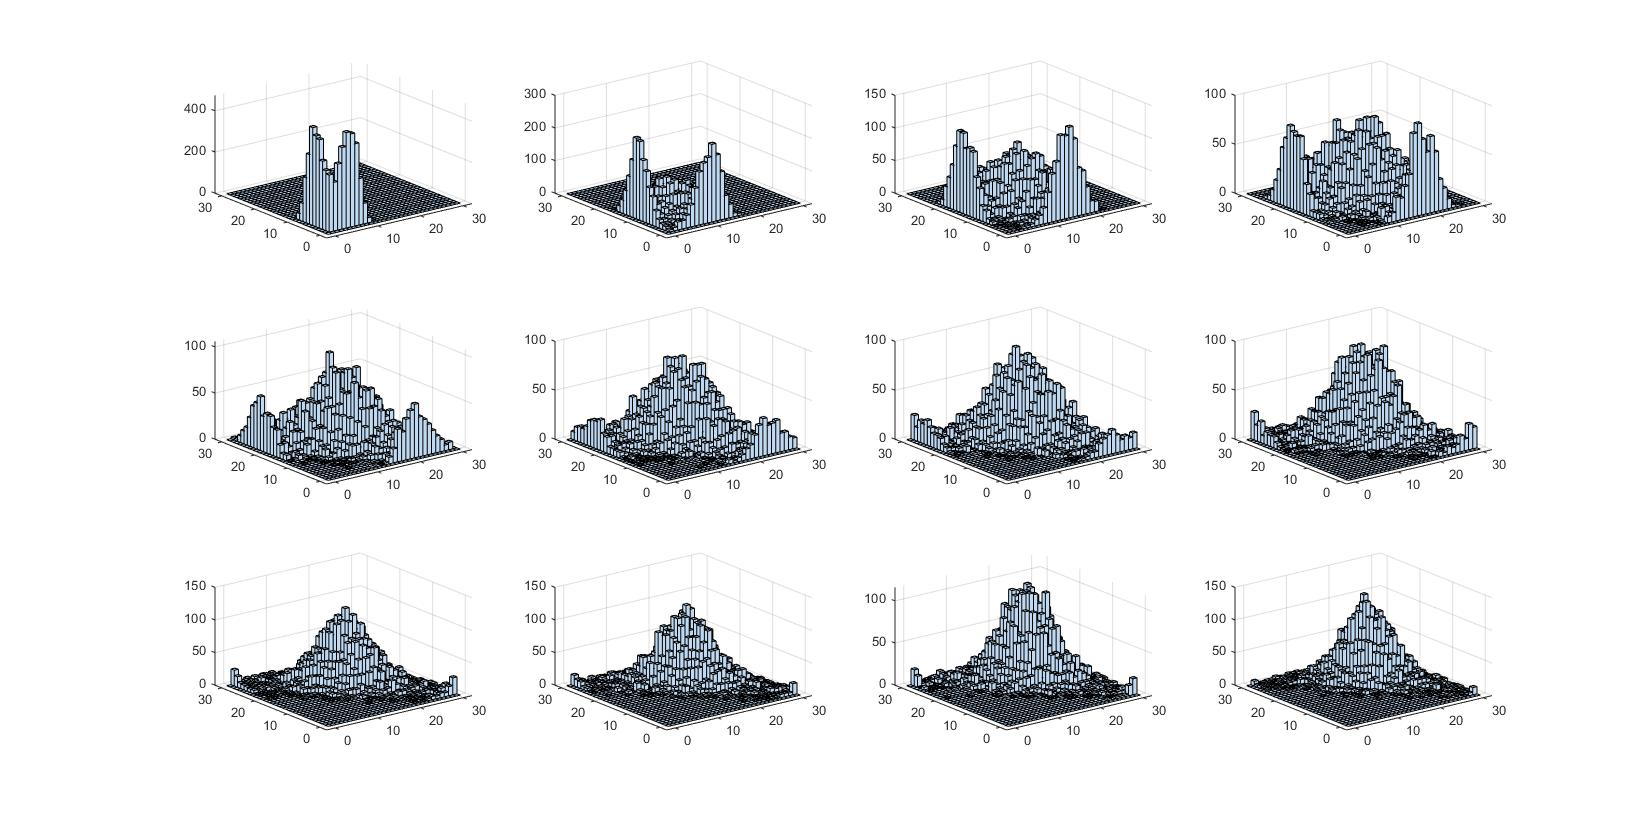
\includegraphics[width=1.7\textwidth]{Figures/figure6.jpg}
	\caption{Question 3 - Distribution of state (t=10  to t=120) over time by t=10 increments}
\end{figure}
\end{landscape}





\end{document}
